\section{Classification and Comparative Study}
\label{sec:comparison}

In order to provide the reader with a quick preview of the generators and thus to enable finding the target solutions easily, we start the survey with a  classification and comparative study of the existing tools. In general, there are various ways to classify them. We first provide an overview of the approaches used in related work after which we then introduce our approach. As mentioned in the Introduction, since this survey is unique in terms of scope and new tools related to Big Data processing, our classification and comparative strategy would differ as well.

The graph data generators can be classified according to various criteria. For example,~\cite{DBLP:conf/sdm/ChakrabartiZF04} introduces two categories -- degree-based and procedural generators. Given a degree distribution (typically following a power law), \emph{degree-based generators} (e.g., Barabasi-Albert model~\cite{Barabasi99emergenceScaling}) try to find a graph that matches it, but without giving any insights about the graph or trying to match other criteria (like, e.g., small diameter, eigenvalues etc.). On the other hand, \emph{procedural generators} (e.g., R-MAT~\cite{DBLP:conf/sdm/ChakrabartiZF04}) try to find simple mechanisms to generate graphs that match a property of the real graphs and, typically, the power law degree distribution.

Paper~\cite{Chakrabarti:2006:GML:1132952.1132954} introduces five categories of graph models that can be synthesized: (1) \emph{random graph models} (e.g., Erd\"{o}s-R\'{e}nyi~\cite{Erdos:1960}) generated by a random process, (2) \emph{preferential attachment models} (e.g., Barabasi-Albert model) which try to model the power law from the preferential attachment viewpoint, (3) \emph{optimization-based models} (e.g., HOT model~\cite{PhysRevLett.84.2529}) resulting from the idea that power laws can result from resource optimizations and tolerance to risks, (4) \emph{tensor-based models} (e.g., R-MAT) targeting a trade-off between low number of model parameters and efficiency, and (5) \emph{internet-specific models} corresponding to hybrids using ideas from the other categories in order to suit the specific features of the graphs.

The type of the generator can also be influenced by the benchmark involving it, whereas we can distinguish, e.g., \emph{domain-specific} benchmarks, \emph{application-specific} benchmarks, \emph{workload-driven} benchmarks,  \emph{microbenchmarks} etc.


%\paragraph{Erd\"{o}s-R\'{e}nyi} One of the first and still very popular approaches with lots of variations and modifications is the random graph model proposed in~\cite{Erdos:1960}. Given a positive integer $n$ and a probability value $0 \leq p \leq 1$, the graph $G(n,p)$ is an undirected graph on $n$ vertices whose edges are chosen s.t. for all pairs of vertices $u,v$ there is an edge $(u,v)$ with probability $p$.
%
%\paragraph{Barabasi-Albert} The Barabasi-Albert (BA) model~\cite{Barabasi99emergenceScaling} proposes that structure emerges in network topologies as the result of two processes -- growth and preferential attachment. The BA model starts with a small set of nodes and grows the network as nodes and edges are added over time. Preferential attachment is based on the idea that the probability of connecting to a node is proportional to the current degree of that node (i.e., ``the rich get richer'').
%
%\paragraph{HOT} The highly optimized tolerance (HOT)~\cite{PhysRevLett.84.2529} model is introduced  using a ``forest fire'' example as follows: Suppose we have a forest which is prone to forest fires. Each portion of the forest has a different chance of starting the fire. We wish to minimize the damage by assigning (a limited amount of) resources such as firebreaks at different positions in the forest. More precisely, we have $n$ possible events, each with an associated probability $p_i, 1 \le i \le n$. Each event can lead to some loss $l_i$, which is a function of the resources $r_i$ allocated for that event $(l_i = f (r_i))$, whose total number is limited ($\sum_i r_i \le R$ for some given $R$). The aim is to minimize the expected cost $\sum_i p_i l_i$. The authors show that resource placement is related to the probability distribution $p_i$ by a power law and the probability of events which cause a loss greater than some value $k$ is related to $k$ by a power law too.
%
%
%\paragraph{R-MAT} The R-MAT (Recursive MATrix)~\cite{DBLP:conf/sdm/ChakrabartiZF04} model can be used to create graphs with community structure, power law degree distributions, and a small diameter. It generates weighted, directed and bipartite graphs. Graph generation is modeled with a matrix recursion -procedure in which the adjacency matrix (empty at the beginning) is recursively subdivided into four equal-sized partitions and edges are distributed across the partitions with unequal probabilities.


%In Figure~\ref{fig:classification} ...
%
%\begin{figure}
%\centering
%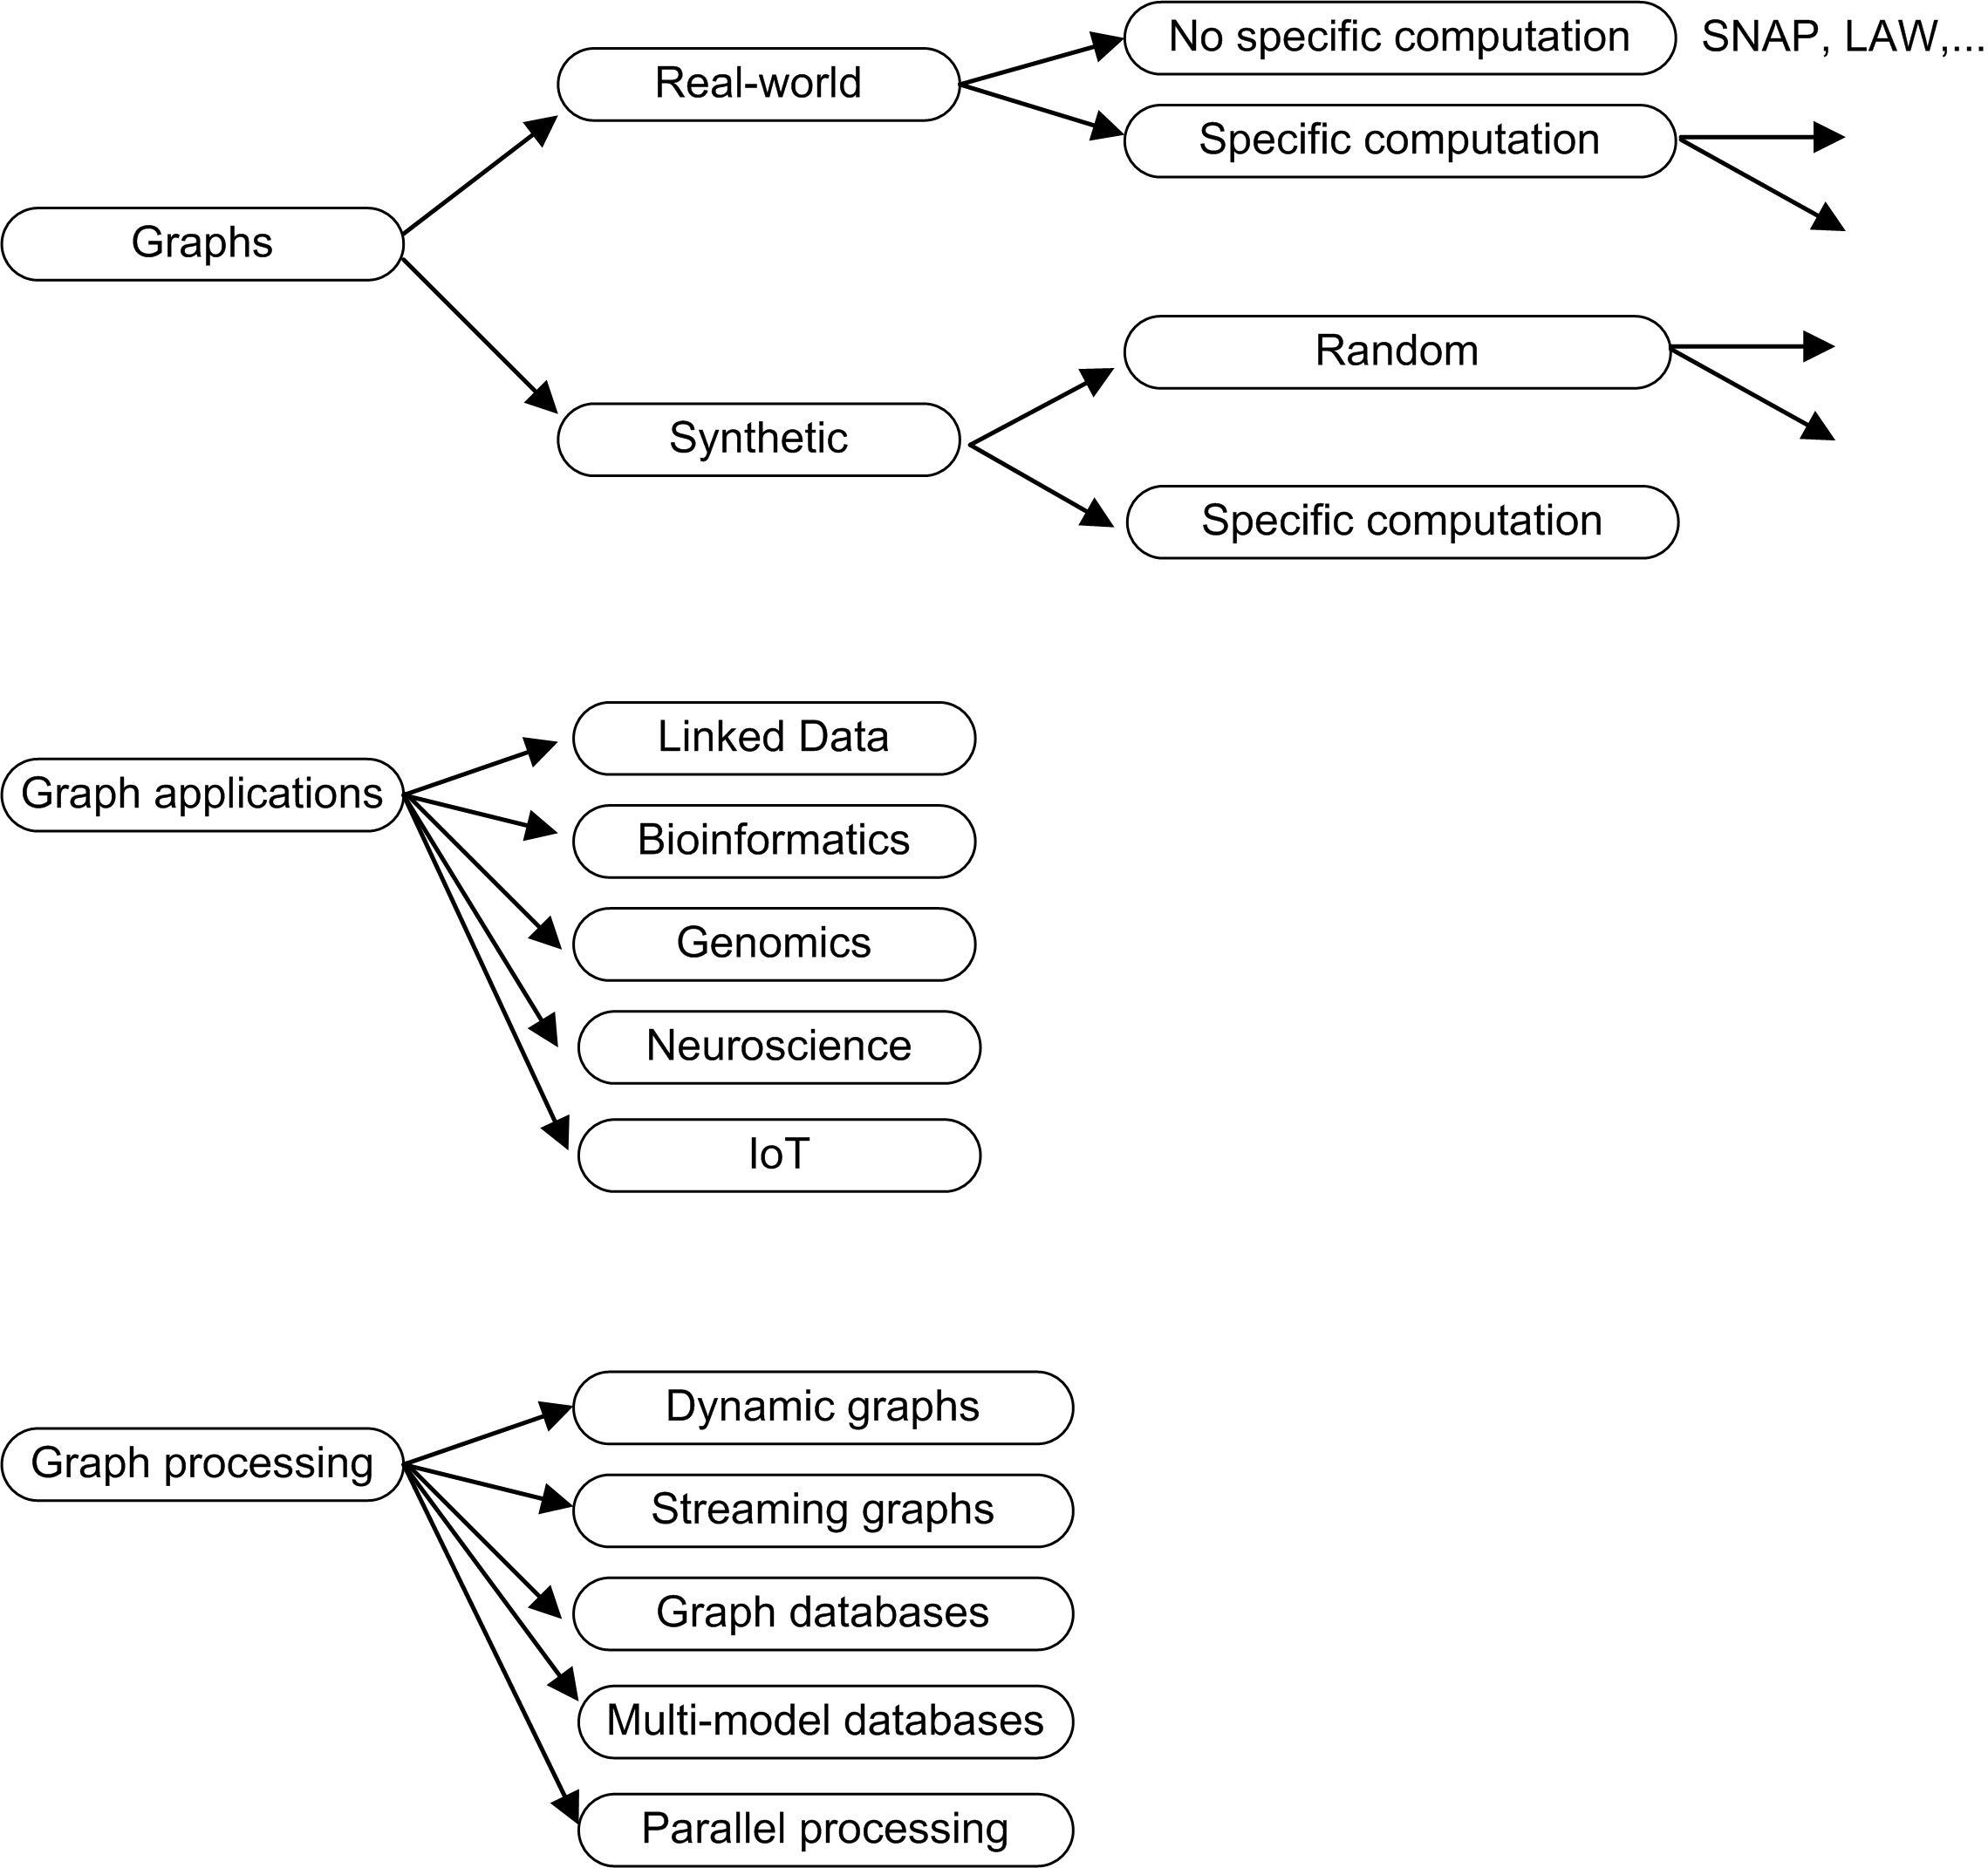
\includegraphics[width=0.8\textwidth]{classification.png}
%\caption{Classification of graph data generators}
%\label{fig:classification}
%\end{figure}

\subsection{Classification}

\TODO{Add info to all three tables.}

At first we classify the generators on the basis of the respective application domains or user communities. In particular we distinguish (1) general graphs, (2) Semantic Web, (3) graph databases, (4) social networks, (5) graph analytics, and (6) graph data steaming. The selected classes are not rigorously defined (e.g., they are not disjoint as we will show later), but they correspond to the currently most active research areas. Thus we believe that they form a natural first acquaintance for the reader.

In Tables~\ref{tab:comparisonCharacteristicsA},~\ref{tab:comparisonCharacteristicsB}   we overview the key characteristics of the data generators clustered according to the respective application domains.\footnote{``GDBs'' stands for graph databases, ``SNs'' stands for social networks, ``An.'' stands for graph analytics, ``St.'' stands for graph streaming.} In particular, we show:

\begin{itemize}
\item Characteristics of the domain -- its \textit{type} (fixed, specified using a schema, or extracted from input data) and the particular \textit{target} domain, or, in case of a generic tool, the chosen sample domain,
\item Characteristics of \textit{read}/\textit{update} operations (if provided), i.e., whether the set of operations is fixed/generated, if it involves operation mixes (i.e., sets/sequences of operations), or if templates of operations are supported.
\item Key configuration options:
  \begin{itemize}
    \item whether the generator deals only with structure, or also with \textit{properties} of the graph,
    \item supported types of \textit{distributions} used for generating of the data,
    \item \textit{output format} of the produced graph, and
    \item  whether the generator is \textit{distributed} and thus enables more efficient data generation.
  \end{itemize}
\end{itemize}


\begin{sidewaystable}
\scriptsize
\centering
\tbl{Key characteristics of the generators (part A)} {
\begin{tabular}{| c | p{2.2cm} | p{2cm} |  p{2.2cm} | l |  l | l | p{3cm} | p{1.4cm} | l | }
 \hline
           &   & \multicolumn{2}{c}{\textbf{Domain}}
               & \multicolumn{2}{|c|}{\textbf{Operations}}
               & \multicolumn{4}{c|}{\textbf{Configuration}}
               \\ \hline
           &  \textbf{Generator}
               & \textbf{Type}
               & \textbf{Target / sample}
               & \textbf{Read}
               & \textbf{Update}
               & \textbf{\rot{Properties}}
               & \textbf{Distributions}
			   & \textbf{Output}
               & \textbf{\rot{Distributed\ }}
               \\ \hline
\hline   % ====================== general graphs
\multirow{7}{*}{\rot{\textbf{General}}}
  & \cite{barabasi1999emergence} & fixed & & Y & N & Y &  & edge-list &  N  \\
\cline{2-10}
   & R-MAt & fixed & & Y & N & Y & power-law & edge-list &  N  \\
\cline{2-10}
  & GraphGen & fixed & N & Y & N & Y&  & & N   \\
\cline{2-10}
  & Graph 500  & fixed & Various Domains& Y & N & Y & power-law & &  Y  \\
\cline{2-10}
  & BTER & fixed & N &   N &  & N & user-defined & edge-list & Y  \\
\cline{2-10}
  & Darwini & fixed & N &   N &  & N & user-defined &  edge-list & Y   \\
%  & Watts-Strogatz~\cite{watts1998collective} & fixed & & Y & N & Y &  & &  N  \\
%\cline{2-10}
\hline
\hline %  ======================  Semantic web
\multirow{20}{*}{\rot{\textbf{Semantic web}}}
 & LUBM & fixed & university  & fixed & N & Y & random (LCG) &  RDF & N   \\
\cline{2-10}
 & LBBM & extracted & Lehigh University BibTeX  & N & N & Y & Monte Carlo &  RDF & N   \\
\cline{2-10}
 & UOBM & fixed & university  & fixed & N & Y & random &  RDF & N   \\
\cline{2-10}
 & IIMB & fixed & movies  & N & N & Y & random &  RDF & N   \\
\cline{2-10}
 & BSBM & fixed & e-commerce  & fixed & N & Y & mostly normal &  RDF, relational & N   \\
\cline{2-10}
 & SP$^2$Bench & fixed & DBLP  & fixed & N & Y & based on DBLP  & RDF & N   \\
\cline{2-10}
 & \cite{Duan:2011:AOC:1989323.1989340} & extracted & -- & N & Y &N & -- &  RDF & N    \\
\cline{2-10}
 & DBPSB & extracted & DBpedia &  templates & N & Y & random &  RDF & N   \\
\cline{2-10}
 & LODIB & fixed & e-commerce &  N & N & Y & 44 types &  RDF & N   \\
\cline{2-10}
 & SIB & fixed & social network &  mixes & mix & Y & from real-world data &  RDF & N   \\
\cline{2-10}
 & Geographica & fixed & OpenStreetMap  & fixed + templates  & N & Y & -- &  RDF & N   \\
\cline{2-10}
 & WatDiv & schema-driven & user-defined  & templates & N & Y & uniform, normal, Zipfian &  RDF & N   \\
\cline{2-10}
 & RBench & extracted & DBLP, Yago  & templates & N & Y & from real-world data &  RDF & N  \\
\cline{2-10}
 & LDBC SPB & fixed & media  & mixes & N & Y & power law, skewed values, value correlation &  RDF & N  \\
\cline{2-10}
 & LinkGen & schema-driven & user-defined & templates & Y  & N & Gaussian, Zipfian& RDF & N\\
\hline
\end{tabular} }
\label{tab:comparisonCharacteristicsA}
\end{sidewaystable}

\begin{sidewaystable}
\scriptsize
\centering
\tbl{Key characteristics of the generators (part B)} {
\begin{tabular}{| c | p{2.2cm}| p{2cm} |  p{2.2cm} | l |  l | l | p{3cm} | p{1.4cm} | l | }
 \hline
           &   & \multicolumn{2}{c}{\textbf{Domain}}
               & \multicolumn{2}{|c|}{\textbf{Operations}}
               & \multicolumn{4}{c|}{\textbf{Configuration}}
               \\ \hline
           &  \textbf{Generator}
               & \textbf{Type}
               & \textbf{Target / sample}
               & \textbf{Read}
               & \textbf{Update}
               & \textbf{\rot{Properties}}
               & \textbf{Distributions}
			   & \textbf{Output}
               & \textbf{\rot{Distributed\ }}
               \\ \hline
\hline  % ======================  graph databases
\multirow{7}{*}{\rot{\textbf{GDBs}}}
  & XGDBench & fixed  & social network  & fixed & Y & Y & power-law &  MAG &  Y  \\
\cline{2-10}
  & gMark & schema-driven (internal schema) &  user-defined  & generated &  N  & Y & uniform, normal, zipfian &  N-triples & N    \\
\cline{2-10}
  & graphGen & pattern-driven (Cypher schema) & user-defined  & -- & -- & Y & -- &  property graphs & N   \\
\hline
\hline %  ======================   social networks
\multirow{8}{*}{\rot{\textbf{SNs}}}
 & \cite{Barrett:2009:GAL:1995456.1995598} & fixed & social network & N & N & Y & simulation-driven & impl. not available &  -- \\
\cline{2-10}
 & \cite{Yao2011} & fixed & social network & N & N & N & power-law & impl. not available & --  \\
\cline{2-10}
 & LinkBench & fixed & social network & Y & Y & Y & Facebook & impl. not available & -- \\
\cline{2-10}
 & S3G2 & fixed & social network  & N & N  & Y & Facebook  & CSV, RDF & Y   \\
\cline{2-10}
 & \cite{Sukthankar-SocialInfo2014} & schema-driven & social-network & N & N & Y & power-law & CSV & N   \\
\cline{2-10}
 & LDBC SNB  & fixed & social network &  generated & Y  & Y & Facebook &  CSV, RDF & Y     \\
\cline{2-10}
  & \cite{Nettleton2016} & schema-driven & social network & N & N & Y & power-law & impl. not available & --  \\
%\cline{2-10}
% & SNG  & Y & Y &   N &  & Y & power-law & ? &  ?   \\
%\cline{2-10}
% & Forest Fire  & N & Y   & N &  & N & power-law &  ? & N   \\
\hline
\hline   % ======================   graph analytics
\multirow{3}{*}{\rot{\textbf{Ana.}}}
  & HPC Scalable Graph Analysis & fixed & & Y & N& N& uniform & & N   \\
\cline{2-10}
  & Graphalytics & extracted & social network & Y& N& power law & & & N   \\
\hline
\hline   %  ======================  streaming
\multirow{2}{*}{\rot{\textbf{St.}}}
  & S2Gen & schema-driven & Social Network & Y & N & N & user-defined & RDF & N     \\
\cline{2-10}
  & RSPLab & schema-driven & Agnostic & Y & Y & N & user-defined & RDF & N     \\
%\cline{2-10}
%  & & & & & & & &  &   \\
\hline
\end{tabular} }
\label{tab:comparisonCharacteristicsB}
\end{sidewaystable}

As we can see ... \TODO{Add a summary.}

\subsection{Overlapping}

As we have mentioned, the basic classification that we have used in this paper
is  based on a relatively vague division of the generators on the basis of the
current application domains or research areas. In addition, some of the
generators are either general or have features applicable in other domains. So
the classes can overlap, as depicted in Table~\ref{tab:overlapping}.

\begin{table}[h]
\scriptsize
\centering
\tbl{Overlapping of classes of generators} {
\begin{tabular}{| c | l | l | l | l | l | l | l | }
 \hline
           &  \textbf{Generator}
               & \textbf{\rot{General}}
               & \textbf{\rot{Semantic Web}}
               & \textbf{\rot{Graph databases\ }}
               & \textbf{\rot{Social networks}}
               & \textbf{\rot{Analytics}}
               & \textbf{\rot{Steaming}}
               \\ \hline
\hline   % ====================== general graphs
\multirow{6}{*}{\rot{\textbf{General}}}
  & \cite{barabasi1999emergence} & {\bf x} & & & & & \\
\cline{2-8}
   & R-MAt    & {\bf x} & & & & & \\
\cline{2-8}
  & GraphGen  & {\bf x} & & x & & & \\
\cline{2-8}
  & Graph 500 & {\bf x} & & & & & \\
\cline{2-8}
  & BTER      & {\bf x} & & & & & \\
\cline{2-8}
  & Darwini   & {\bf x} & & & & & \\
\hline
\hline %  ======================  Semantic web
\multirow{15}{*}{\rot{\textbf{Semantic web}}}
 & LUBM  & & {\bf x} & & & & \\
\cline{2-8}
 & LBBM  & & {\bf x} & & & & \\
\cline{2-8}
 & UOBM  & & {\bf x} & & & & \\
\cline{2-8}
 & IIMB & & {\bf x} & & & & \\
\cline{2-8}
 & BSBM & & {\bf x} & & & & \\
\cline{2-8}
 & SP$^2$Bench & & {\bf x} & & & & \\
\cline{2-8}
 & \cite{Duan:2011:AOC:1989323.1989340} & & {\bf x} & & & & \\
\cline{2-8}
 & DBPSB & & {\bf x} & & & & \\
\cline{2-8}
 & LODIB & & {\bf x} & & & & \\
\cline{2-8}
 & SIB & & {\bf x} & & & & \\
\cline{2-8}
 & Geographica & & {\bf x} & & & & \\
\cline{2-8}
 & WatDiv & & {\bf x} & & & & \\
\cline{2-8}
 & RBench & & {\bf x} & & & & \\
\cline{2-8}
 & LDBC SPB & & {\bf x} & & & & \\
\cline{2-8}
 & LinkGen & & {\bf x} & & & & \\
\hline
\hline  % ======================  graph databases
\multirow{3}{*}{\rot{\textbf{GDBs}}}
  & XGDBench & & & {\bf x} & x & & \\
\cline{2-8}
  & gMark & & x & {\bf x} & x & & \\
\cline{2-8}
  & graphGen & & & {\bf x} & & & \\
\hline
\hline %  ======================   social networks
\multirow{7}{*}{\rot{\textbf{SNs}}}
 & \cite{Barrett:2009:GAL:1995456.1995598} & & & & x & & \\
\cline{2-8}
 & \cite{Yao2011}  & & & & {\bf x} & & \\
\cline{2-8}
 & LinkBench  & & & x & {\bf x} & & \\
\cline{2-8}
 & S3G2  & & x & x & {\bf x} & & \\
\cline{2-8}
 & \cite{Sukthankar-SocialInfo2014}  & & & & {\bf x} & & \\
\cline{2-8}
 & LDBC SNB   & & x & x & {\bf x} & & \\
\cline{2-8}
  & \cite{Nettleton2016}  & & & & {\bf x} & & \\
\hline
\hline   % ======================   graph analytics
\multirow{2}{*}{\rot{\textbf{An.}}}
  & HPC Scalable Graph Analysis  & & & & & {\bf x} & \\
\cline{2-8}
  & Graphalytics & & & & & {\bf x} & \\
\hline
\hline   %  ======================  streaming
\multirow{2}{*}{\rot{\textbf{St.}}}
  & S2Gen & & & & & & {\bf x}\\
\cline{2-8}
  & RSPLab & & & & & & {\bf x} \\
%\cline{2-8}
%  & & & & & & \\
\hline
\end{tabular} }
\label{tab:overlapping}
\end{table}

\TODO{Extend summary.}
For example, some social network graph generators such as the LDBC-SNB, S3G2 or
LinkBench, can be used to test graph databases. In the case of the first two,
even though they are designed not to be specific to any type of technology,
they graph databases are their main target.  Additionally, they also provide serializers for
RDF, thus they can also be used to test RDF systems. 

In the case of LinkBench, nothing prevents the user to load the generated graph
in a graph database (Facebook uses a MySQL in that paper) to
test a workload similar to Facebook and extend and complement it with more
graphy queries like those in LDBC-SNB. 

